\title{\vspace{-2cm} PHY102: Conceptual and Procedural Understanding\\\vspace{0.25cm} {Written examination}}
\author{}
\date{\vspace{-2cm} 4th May, 2018}

\maketitle
\vspace{-1.5cm}
\begin{center}
\hrulefill\\
\textbf{Instructions:}

\begin{itemize}
\item \textbf{Read the question paper carefully!}
\item The total duration of the written exam is \textbf{90 minutes}.
\item You are required to return the question paper with your answer sheet.
\item \textbf{No} electronic devices of any kind will be allowed during the examination.
\item Multiple choice questions and sketches must be marked on the question paper \textbf{clearly}.
\end{itemize}
\vspace{-0.9cm}
\hrulefill
\end{center}
\vspace{-0.9cm}
\section*{Multiple Choice Questions \hfill (5 marks)}

\begin{enumerate}
\item What is the distance between two successive divisions on the Vernier scale of a Vernier caliper of least count 0.02 mm?
\begin{enumerate}
\item 1 mm
\item 1/50 mm
\item 49/50 mm \hfill \textbf{(1 mark)}
\end{enumerate}


% \item With water, the colour red of a rainbow is observed at $42^\circ$. Supposing instead you had an acid solution (of density 1.5 g/cc). Red will now appear at:
% \begin{enumerate}
% \item An angle greater than $42^\circ$,
% \item An angle less than $42^\circ$,
% \item The same angle.\hfill \textbf{(1 mark)}
% \end{enumerate}


\item Why was a lens used in the Formation of Rainbow experiment? \hfill \textbf{(1 mark)}

\begin{enumerate}
\item To concentrate the light from the bulb onto the drop.
\item To make the light rays from the source parallel.
\item To create a point source from an extended source.
\end{enumerate}

\item You are given three laser sources which emit light of wavelengths $\lambda_1$, $\lambda_2$ and $\lambda_3$. On passing them through a fixed grating -- keeping all else constant -- the pattern of bright spots on the screen is observed as shown in Figure \ref{lambdaGratings}. Which of the following is true? \hfill \textbf{(2 marks)}

\renewcommand{\figurename}{\hspace{4cm} Figure}


\begin{figure}[!htb]\hspace{2cm}
\centering
\hspace{2cm}
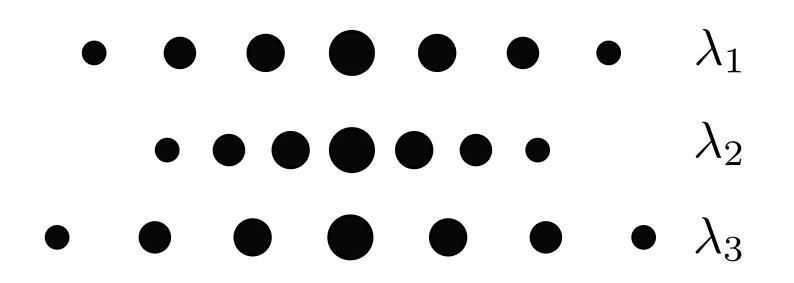
\includegraphics[width=0.5\textwidth]{q10.png}%
\hfill\caption{How are the $\lambda$s related?}
\label{lambdaGratings}
\end{figure}
\vspace{-4cm}
\begin{enumerate}
\item $\lambda_1 > \lambda_2 > \lambda_3$
\item $\lambda_1 < \lambda_2 < \lambda_3$
\item $\lambda_2 < \lambda_1 < \lambda_3$
\item $\lambda_2 > \lambda_1 > \lambda_3$
\item $\lambda_2 > \lambda_3 > \lambda_1$
\end{enumerate}
\vspace{0.5cm}


\renewcommand{\figurename}{Figure}
\newpage
\item Three identical $12$ V bulbs (rated at 21W) are arranged in a circuit as indicated in Figure \ref{bulbGlow}. Which of the following is/are true? \hfill \textbf{(1 mark)}


\renewcommand{\figurename}{\hspace{5cm} Figure}
\vspace{-0.5cm}
\begin{figure}[!htb]
\hspace{4cm}
\centering
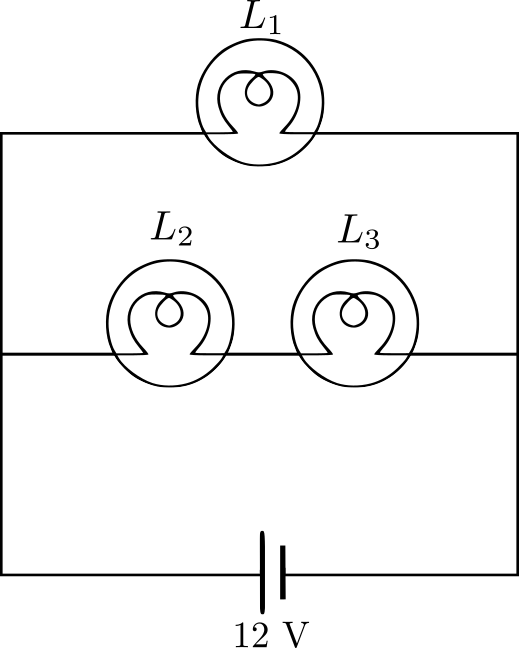
\includegraphics[width=0.25\textwidth]{q1.png}
\caption{}
\label{bulbGlow}
\end{figure}

\vspace{-5cm}

\begin{enumerate}
\item $L_1$ glows the brightest,
\item $L_2$ and $L_3$ glow equally brightly,
\item $L_2$ glows brighter than $L_3$,
\item $L_1$ and $L_2$ glow equally brightly.
\end{enumerate}

\vspace{2.5cm}
\renewcommand{\figurename}{Figure}

\section*{Short Answer Questions \hfill (10 marks)}



% \item State Babinet's principle and explain it with the help of an example, describing in detail the diffraction patterns observed.  \hfill \textbf{(1 mark)}


% \item What are the smallest and largest lengths that can be theoretically measured by diffraction using light of a wavelength 532 nm. Justify your answer. \hfill \textbf{(2 marks)}



\item Why does the intensity of light of a point source fall off as the inverse square of the distance from the source? \hfill \textbf{(2 marks)}


\item If $f'_0$ is the fundamental frequency of a massive spring with one end clamped, and $f_0$ is the fundamental frequency of the same spring with both ends clamped, explain why $f_0 = 2 f'_0$. You may use a suitable analogy if required. \hfill \textbf{(2 marks)}

% \item A single slit of width $a$ is placed in the way of a laser. The normalised intensity of the diffraction pattern is plotted against a function ($\pi a \sin\theta / \lambda$) of the angular separation $\theta$ as shown in Figure \ref{intensityPattern}. On the same figure (Figure \ref{intensityPattern}), sketch the pattern if the slit width is doubled. \hfill \textbf{(1 mark)}

% \begin{figure}[!htb]
% \centering
% 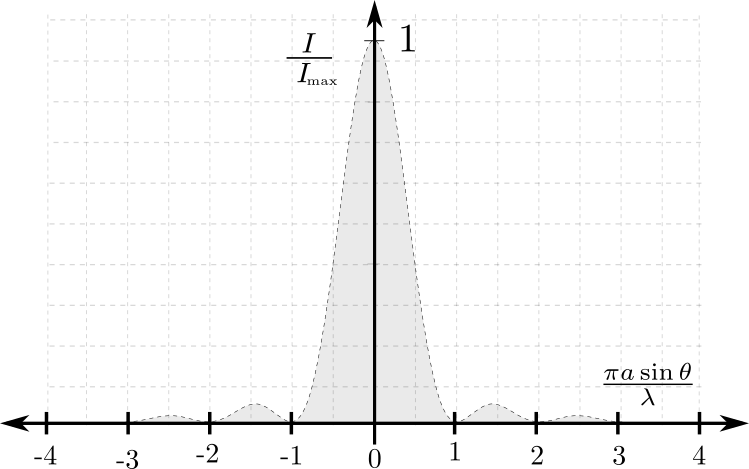
\includegraphics[width=0.85\textwidth]{q8.png}
% \caption{Sketch the new pattern on the graph.}
% \label{intensityPattern}
% \end{figure}


\item Suggest a method to increase the intensity of the light falling on the drop in the Formation of Rainbow experiment, assuming that we cannot change the bulb or power supply. You have at your disposal many lenses of different sizes, focal lengths and powers. \hfill \textbf{(2 marks)}

\item Sketch the following graphs for a simple pendulum that is left from rest at a small angle $A$.

\begin{enumerate}
\item Position vs. Time
\item Velocity vs. Time 
\item Acceleration vs. Time \hfill \textbf{(2 marks)}
\end{enumerate} 

\item Roughly sketch a graph of the \textit{residence time} of the above-mentioned pendulum over a single cycle in Figure \ref{resGraph}. The residence time is defined as the amount of time ($\Delta t$) that the pendulum spends in a region of space ($\Delta x$). \hfill \textbf{(2 marks)}

\begin{figure}[!htb]
\centering
\begin{subfigure}[b]{0.5\textwidth}
\centering
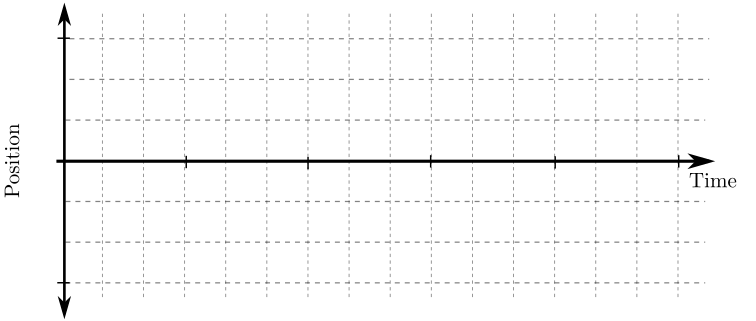
\includegraphics[width=\textwidth]{q11.png}
\caption{Question 9(a)}
\end{subfigure}%
\begin{subfigure}[b]{0.5\textwidth}
\centering
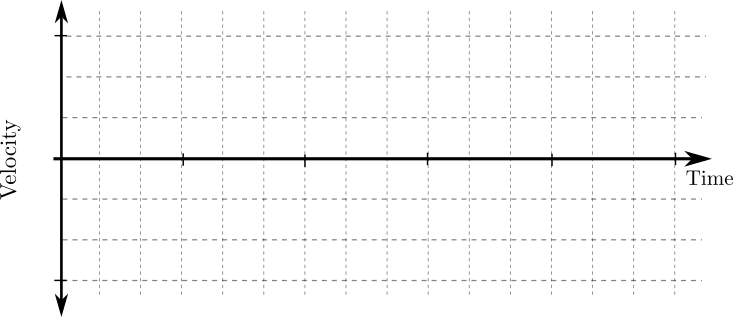
\includegraphics[width=\textwidth]{q12.png}
\caption{Question 9(b)}
\end{subfigure}
\begin{subfigure}[b]{0.5\textwidth}
\centering
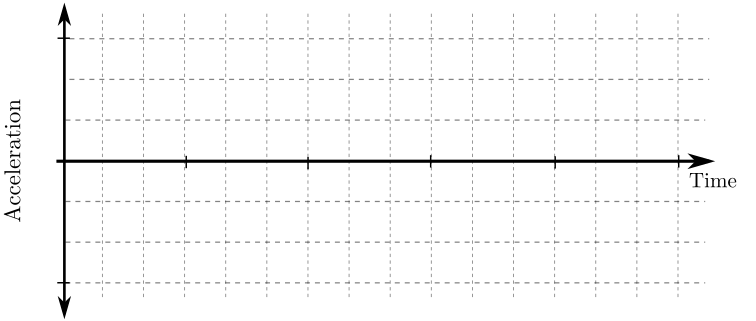
\includegraphics[width=\textwidth]{q13.png}
\caption{Question 9(c)}
\end{subfigure}
\end{figure}



\begin{figure}[!htb]
\centering
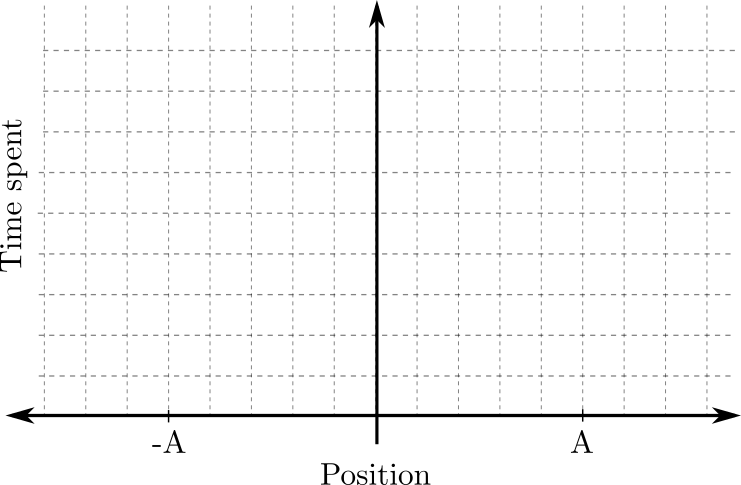
\includegraphics[width=0.85\textwidth]{q7.png}
\caption{Sketch a graph of residence time versus position.}
\label{resGraph}
\end{figure}

\newpage
~\\
~\\
\newpage
\section*{Long Answer Questions \hfill (15 marks)}



\item You are conducting an experiment to measure the time period of a simple pendulum using a \textbf{stopwatch}. At which point of the trajectory would you start counting the number of cycles? 

Now suppose instead that you are using a \textbf{digital sensor} to detect the pendulum's position. At which point of the pendulum's trajectory would you place such a sensor if you want to count the number of cycles?

Justify your answer in both the above cases. (\textbf{Hint:} You can use your answer from Question (9).)  \hfill \textbf{(3 marks)}


\item Why was soap solution used in the Surface Tension experiment? How much soap should one ideally use for the experiment? Justify your answer. \hfill \textbf{(3 marks)}



\item In the experiment for the Characterisation of an Incandescent Lamp, the circuit is set up as shown in Figure \ref{incandCirc} with a 12V lamp rated at 21W. However, the bulb is found to not glow. Explain why this happens.  \hfill \textbf{(3 marks)}

\begin{figure}[!htb]
\centering
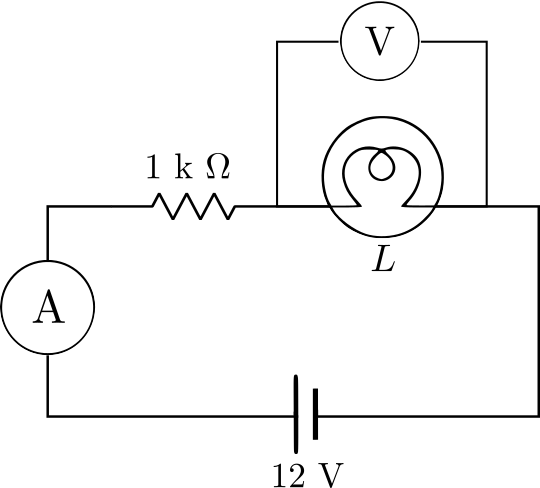
\includegraphics[width=0.25\textwidth]{q2.png}
\caption{Explain why the bulb does not glow.}
\label{incandCirc}
\end{figure}


\item Design an experiment to find the resistance of a fuse (rated 500 mA). You are provided with a power supply ($0-5$V), two digital multimeters, and a resistance ladder. Make sure you mention \textbf{all} necessary details, including the settings of the multimeter, and provide a circuit diagram. \hfill \textbf{(3 marks)}



% \item The displacement of the free end of a slinky spring clamped at its upper end and oscillating vertically is given by 

% \begin{equation*}
% Y = A e^{-\left(\frac{b}{2m}\right) t}\cos{\omega t}
% \end{equation*}

% \noindent where $A$, $b$, $\omega$ and $m$ are constants and $t$ is time. Design an experiment to determine the factor $b/m$. Mention all the stages of data collection and interpretation, including the number of readings you will take and why, as well as graphs you will plot (if any). \hfill \textbf{(5 marks)}


% \item When drops are formed on a plane surface due to Surface Tension, the following relations are found to hold true:

% \begin{equation*}
% \begin{aligned}
% T &= k \cdot m \cdot g\\
% T &= C \cdot r^x \cdot d^y
% \end{aligned}
% \end{equation*}

% \noindent where $k$ and $C$ are constants, $r$ is the radius of the formed drop and $d$ the density of the solution. $x$ and $y$ are numbers. Design an experiment to find $x$. You are provided with a \textbf{glass plate}, \textbf{soap powder}, a \textbf{weighing balance} and \textbf{beakers}. You may include other objects if required.  \hfill \textbf{(3 marks)}



% \item Describe the diffraction pattern you would obtain using a Double Helix, indicating clearly which parameter of the Double Helix governs which parameter in the pattern. \hfill \textbf{(3 marks)}



\item Sketch the IV Characteristics of the circuits represented in Figure \ref{IVChar}. State the units on the axes of the graphs, as well as the rough values of voltage and current which characterise the circuit. \hfill \textbf{(3 marks)}

\begin{figure}[!htb]
\centering \hfill
\begin{subfigure}[b]{0.5\textwidth}
\centering
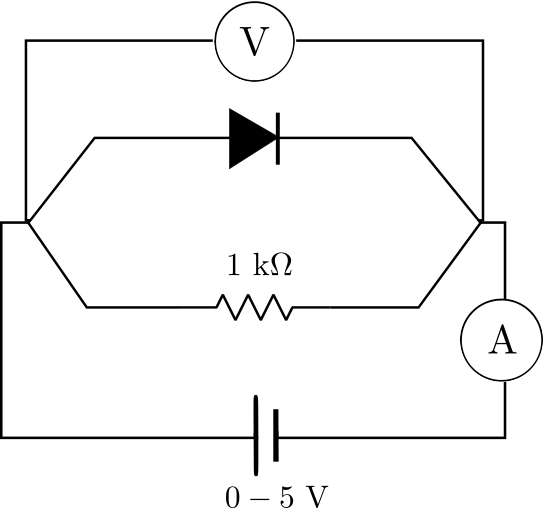
\includegraphics[width = 0.5\textwidth]{q3.png}
\end{subfigure}\hfill
\begin{subfigure}[b]{0.5\textwidth}
\centering
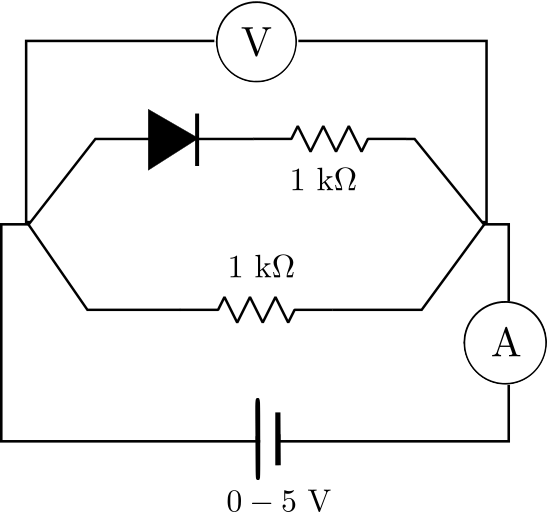
\includegraphics[width = 0.5\textwidth]{q4.png}
\end{subfigure}%
\hfill
\caption{Question 14 | Sketch the IV Characteristics}
\label{IVChar}
\end{figure}



% \begin{figure}[!htb]
% \centering
% 
\includegraphics[width=0.85\textwidth]{q9.png}
% \vspace{1.5cm}
% \caption{Sketch the pattern for a thin wire of thickness 1 mm.}
% \label{diffractionSlit}
% \end{figure}
\end{enumerate}

\begin{figure}[!htb]
\centering
\begin{subfigure}[b]{\textwidth}
\centering
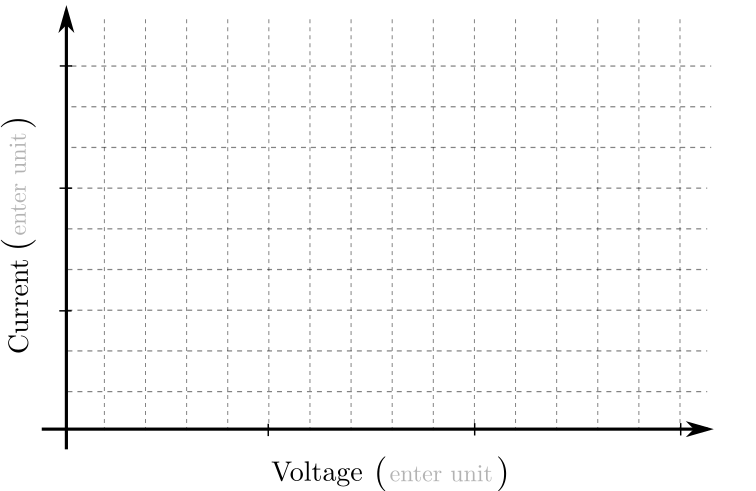
\includegraphics[width=\textwidth]{q6.png}
\caption{Question 14(a)}
\end{subfigure}
\begin{subfigure}[b]{\textwidth}
\centering
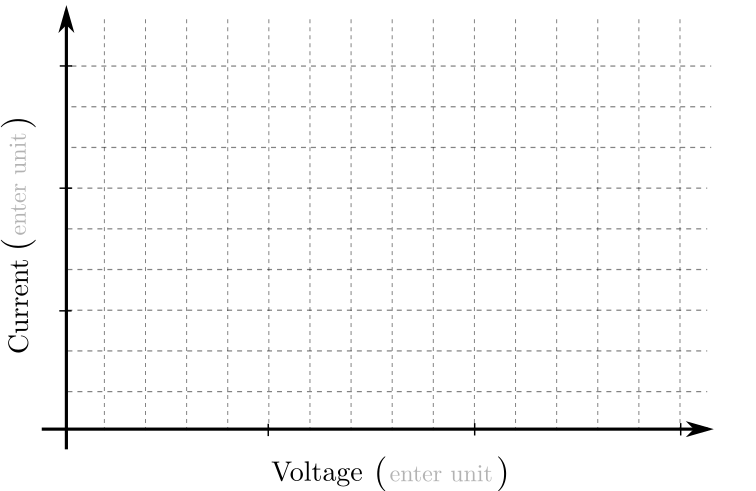
\includegraphics[width=\textwidth]{q6.png}
\caption{Question 14(b)}
\end{subfigure}
\end{figure}